\documentclass[preprint,11pt]{elsarticle}

\usepackage{amsmath}
\usepackage{booktabs}
\usepackage{graphicx}
\usepackage{xcolor}
\usepackage{tikz}
\usetikzlibrary{positioning,arrows.meta,fit,backgrounds}
\usepackage[hidelinks]{hyperref}
\usepackage{url}

\newcommand{\todo}[1]{\textcolor{red}{[TODO: #1]}}

\journal{Computers in Industry}

\begin{document}

\begin{frontmatter}

\title{From detection to action: closing the autonomic loop of a self-coordinated manufacturing line with rule-based and retrieval-augmented LLM planners}

\author[a,b]{Manuel S\'anchez\corref{cor1}}
\ead{mbsanchez@unet.edu.ve}
\author[b]{Ernesto Exposito}
\ead{ernesto.exposito@univ-pau.fr}
\cortext[cor1]{Corresponding author.}
\address[a]{Universidad Nacional Experimental del T\'achira, San Crist\'obal, Venezuela}
\address[b]{Univ Pau \& Pays Adour / E2S UPPA, Laboratoire d'informatique de l'Universit\'e de Pau et des Pays de l'Adour (LIUPPA), EA3000, 64000 Pau, France}

\begin{abstract}
Autonomic architectures for Industry~4.0 promise self-configuring, self-healing and self-optimising production, but published systems often stop at detection. We revisit our own 2020 self-coordinated manufacturing architecture and its simulator, and find that it implements Monitor and Analyze but not Plan, Execute or a Knowledge base: detected conditions only produce a log message. We port the simulator to a headless, tested engine over the Bosch production-line dataset and close the loop with an action space built on the line's parallel twin stations, a symbolic validator, fault injection (step, intermittent and drift faults) and an explicit effect model. We compare rule-based planners with large-language-model (LLM) planners with and without retrieval-augmented operational knowledge, on a local 7B model (Qwen2.5) and a frontier model (Claude Fable~5.1), using a development trace for design and three held-out traces for evaluation. Wiring the original alarms directly to repairs gains nothing on the held-out traces (pooled recovery $+0.02$) while repairing 87 healthy stations per fault scenario. The bottleneck is alarm triage, not planning: a classical adaptive change test recovers 52--54\% of the delay caused by faults, and re-tuning its hyperparameters on the development trace does not improve it. With the 7B model, the retrieval-augmented planner recovers 20\%; with the frontier model the same design recovers 58\%, statistically indistinguishable from the best rule (difference $+0.04$, 95\% interval $-0.01$ to $+0.10$); without retrieved knowledge, the frontier model declines to act at all. On intermittent faults it is ahead of every rule configuration we tried, but this exploratory result rests on 24 scenarios from three traces and its interval reaches zero. Used instead as a veto over the original detector, the frontier model becomes extremely conservative and attributes almost every alarm to a line-wide cause, a structure that the detector imposes on all its alarms. Closing autonomic loops in manufacturing therefore depends more on the Analyze--Knowledge interface than on the capability of the planner.
\end{abstract}

\begin{highlights}
\item The 2020 autonomic architecture detected conditions but never planned or acted.
\item Wiring legacy alarms straight to repairs gains nothing and repairs healthy stations.
\item A classical adaptive change test is a strong baseline for alarm triage.
\item A frontier LLM with retrieved knowledge matches that test but does not beat it.
\item As a veto over batched alarms, the frontier LLM becomes overly conservative.
\end{highlights}

\begin{keyword}
Autonomic computing \sep MAPE-K \sep Industry 4.0 \sep Large language models \sep Retrieval-augmented generation \sep Fault management
\end{keyword}

\end{frontmatter}

% =====================================================================
\section{Introduction}
\label{sec:intro}

Autonomic computing proposes systems that manage themselves through a Monitor--Analyze--Plan--Execute loop over a shared Knowledge base (MAPE-K)~\cite{kephart2003vision,weyns2020introduction}. In manufacturing, this loop is attractive because production lines degrade continuously and human supervision does not scale: a self-healing line would notice a degrading station and reconfigure itself before the delay accumulates.

In 2020 we proposed an architecture for self-coordinated manufacturing processes with self-* properties and evaluated it with a simulator, SSACSimulator, over the Bosch production-line dataset~\cite{sanchez2020selfstar,sanchez2020jii}. Revisiting that code six years later, we found that it implements the Monitor and Analyze phases only. When one of its three detectors fires, the simulator writes \emph{``launching the autonomous cycle for reconfiguration''} to a log panel; no plan is produced and nothing is executed. The loop was announced, not closed.

This paper closes it, and asks what closing it actually requires. Two developments make the question timely. First, large language models (LLMs) are increasingly proposed as planners for industrial decision making, from the control of modular production systems~\cite{xia2023towards} to advanced planning and scheduling~\cite{li2026a4ps}. Second, retrieval-augmented generation (RAG)~\cite{lewis2020rag} offers a natural candidate for the Knowledge component of MAPE-K: instead of a hand-built ontology, the planner retrieves the operational history it needs. Whether either helps, and against which baseline, is an empirical question.

Our contributions are:
\begin{enumerate}
  \item A faithful, tested, headless port of the 2020 simulator, and an analysis of its Analyze layer on the published data: one of the three detectors is unreachable, one is exercised by 0.004\% of the events, and the third fires routinely on a fault-free trace (Section~\ref{sec:revisit}).
  \item The missing Plan and Execute phases: an action space based on the parallel ``twin'' stations of the Bosch line, a symbolic validator, fault injection with three fault shapes, and an explicit, parameterised effect model whose unverifiable assumptions are swept rather than fixed (Section~\ref{sec:loop}).
  \item A comparison of rule-based planners against LLM planners with and without retrieved knowledge, and of a hybrid in which a statistical test triages and the LLM vetoes, on a local 7B model and a frontier model, under a protocol that separates a development trace from three held-out traces (Sections~\ref{sec:planners}--\ref{sec:results}).
  \item Evidence that the bottleneck of closing the loop is alarm triage rather than planning; that, for retrieval-augmented triage, a frontier model matches a well-tuned statistical test where a 7B model does not, and retrieved knowledge is what lets it act at all; and that the structure of the alarms emitted by the detector shapes how a capable model vetoes them (Section~\ref{sec:discussion}).
\end{enumerate}

All code, data-processing scripts, prompts, every model decision with its stated reason, and all results are available (Section~\ref{sec:availability}).

% =====================================================================
\section{Background and related work}
\label{sec:related}

\paragraph{Autonomic computing and self-adaptive systems}
The MAPE-K reference model~\cite{kephart2003vision} structures a self-managing system as a feedback loop around a managed resource. Engineering such loops is the subject of the self-adaptive systems literature~\cite{weyns2020introduction}, which stresses that the Analyze phase must separate genuine change from noise before any adaptation is planned. LLMs have recently been examined as components of such loops: a state-of-the-art review and research roadmap organises their potential uses around the MAPE-K functions~\cite{li2024genai,li2024exploring}; LLM-based agents have been embedded in MAPE-K-based multi-agent systems~\cite{nascimento2023selfadaptive}; and MAPER extends MAPE-K with an LLM-based reasoning component to handle unanticipated runtime situations~\cite{alves2026maper}. Our study differs in placing an LLM inside the loop of an industrial system whose detector we inherit unchanged, and in measuring it against strong non-LLM baselines on held-out data.

\paragraph{Self-* properties in manufacturing}
Our earlier work integrated multi-agent systems, service orientation and autonomic computing for Industry~4.0 process coordination~\cite{sanchez2020selfstar,sanchez2020jii,sanchez2020survey}. The present paper re-examines that architecture empirically rather than proposing a new one.

\paragraph{Change detection}
Detecting a change in the rate of an event stream is a classical problem~\cite{basseville1993detection}. Our strongest rule-based baselines are simple instances: a Poisson test against a static base rate, and a test against the recent history of the same stream.

\paragraph{LLMs and retrieval in industrial decision making}
RAG conditions a language model on documents retrieved for each query~\cite{lewis2020rag}. In manufacturing, LLM agents have been combined with digital twins to plan and control modular production~\cite{xia2023towards} and applied to advanced planning and scheduling~\cite{li2026a4ps}, and a recent review of LLMs for fault diagnosis in smart manufacturing covers, among other roles, retrieval-augmented fusion of industrial knowledge~\cite{thuan2026review}. Our design deliberately includes a strong statistical baseline and control rules that isolate what the LLM contributes beyond them.

% =====================================================================
\section{The 2020 system revisited}
\label{sec:revisit}

\subsection{Simulator and data}
SSACSimulator is a Qt/C++ discrete-event simulator. A process model, derived from the Bosch Production Line Performance dataset~\cite{bosch2016kaggle}, describes 52 stations on four sub-lines plus begin and end nodes, 285 transitions (84 of them main flows), a throughput time of 6\,420~min and 1\,183\,165 cases. Four event traces of 100\,000 transitions each replay recorded piece movements; they span 54 to 168 hours of production.

\subsection{Headless port}
We ported the simulation core (about 1\,440 lines of C++ logic, excluding the graphical user interface) to Python. The port reproduces the original's behaviour as read from its source, including details that change results: thresholds computed in single precision, a 100\,000-event loading limit, and a lenient rule for malformed rows. A fast path advances only the pieces that can leave the system; the original per-tick loop is kept as a test oracle, and a regression test checks that both produce identical detections, decisions and piece lifetimes. A run takes 0.2--0.4~s. The test suite has 87 tests.

\subsection{What the Analyze layer actually does}
The original implements three detectors: a station whose mean transition time exceeds 1.3 times its reference; more than 10\% of stations flagged within one batch of simultaneous events; and a mean piece lifetime exceeding 1.1 times the throughput time. On the first trace, only the second fires (39 alarms). The predicted-failure detector depends on a classifier label that is positive in 15 of 400\,000 events across all traces (0.004\%). The global detector is unreachable: the mean piece lifetime (636~min) is an order of magnitude below its threshold (7\,062~min). Finally, 45 of the 285 transitions have a reference time of zero, so any positive duration flags their station.

Plan, Execute and Knowledge are absent. This is the starting point for the rest of the paper.

% =====================================================================
\section{Closing the loop}
\label{sec:loop}

Figure~\ref{fig:loop} summarises the closed loop. Components added in this work are shaded.

\begin{figure}[t]
\centering
\resizebox{\linewidth}{!}{%
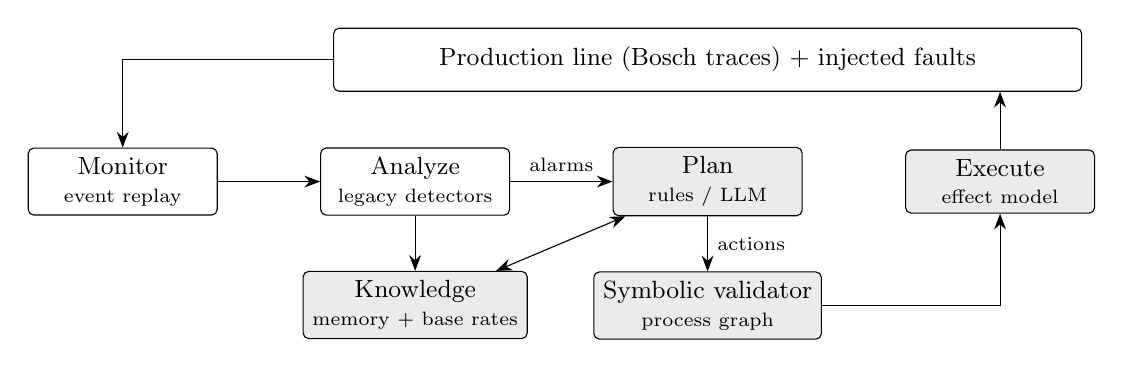
\begin{tikzpicture}[
  node distance=7mm and 13mm,
  box/.style={draw, rounded corners=2pt, minimum width=24mm, minimum height=8mm, align=center, font=\small},
  new/.style={box, fill=black!8},
  >={Stealth[length=2mm]}]
  \node[box] (mon) {Monitor\\[-1pt]\scriptsize event replay};
  \node[box, right=of mon] (ana) {Analyze\\[-1pt]\scriptsize legacy detectors};
  \node[new, right=of ana] (plan) {Plan\\[-1pt]\scriptsize rules / LLM};
  \node[new, right=of plan] (exe) {Execute\\[-1pt]\scriptsize effect model};
  \node[new, below=of ana] (k) {Knowledge\\[-1pt]\scriptsize memory + base rates};
  \node[new, below=of plan] (val) {Symbolic validator\\[-1pt]\scriptsize process graph};
  \node[box, above=of plan, minimum width=95mm] (line) {Production line (Bosch traces) + injected faults};
  \draw[->] (mon) -- (ana);
  \draw[->] (ana) -- node[above, font=\scriptsize]{alarms} (plan);
  \draw[->] (plan) -- node[right, font=\scriptsize]{actions} (val);
  \draw[->] (val.east) -| (exe.south);
  \draw[->] (exe.north) -- (exe.north |- line.south);
  \draw[->] (line.west) -| (mon.north);
  \draw[<->] (k) -- (plan);
  \draw[->] (ana) -- (k);
\end{tikzpicture}}
\caption{The closed MAPE-K loop. White: present in the 2020 system. Grey: added in this work.}
\label{fig:loop}
\end{figure}

\subsection{Twin stations and the action space}
The Bosch line is built from parallel station pairs (and a few triples) that share predecessors and successors and split the load almost evenly; for example, on their main flows stations L0\_S2 and L0\_S3 receive 339\,345 and 334\,054 cases. We identify twins automatically from the overlap of their predecessor and successor sets on main flows: 29 of the 52 stations have one. Diverting a piece from a station to its twin keeps its trajectory consistent, which makes rerouting a physically meaningful action. The action space is \textsc{Reroute}(S, T, $f$), which diverts a fraction $f$ of the pieces entering S to its twin T; \textsc{Restore}(S); \textsc{Maintenance}(S, $d$), which repairs S for $d$ minutes; and \textsc{NoOp}.

\subsection{Symbolic validator}
Every action, from any planner, is checked against the process graph and the current interventions before execution: stations must exist, a reroute target must be a structural twin, reroutes must not form chains, and a station cannot be repaired twice concurrently. The validator never judges whether an action is a good idea, only whether it is admissible.

\subsection{Effect model}
The simulation is trace-driven: start times come from the recorded data and are not shifted; faults and actions act on transition durations, and the lifetime of a piece is the sum of its transition durations. Delay therefore does not propagate as queueing; the model estimates time lost per piece. A Bosch ``transition'' is the time between two station timestamps and mostly measures waiting: its median is 0~min and its 90th percentile 18--30~min, but its 99th percentile reaches 4\,100--5\,900~min. Effects are therefore \emph{additive} and proportional to each station's processing time $\tau_S$ (the median of its transitions of up to 60~min), never multiplicative over a transition that includes days of storage. $\tau_S$ is 6 or 12~min for the eight stations where faults are injected, identical on all traces, and at most 45--57~min over the whole line. The effect model is:
\begin{itemize}
  \item \textbf{Fault} of factor $k$ on S: $+(k(t)-1)\,\tau_S$ on every transition leaving S, where $k(t)$ is a \emph{step} ($k$ from $t_0$), \emph{intermittent} ($k$ for 60~min, 1 for 120~min, repeating) or \emph{drift} (rising linearly from 1 to $k$ over 600~min).
  \item \textbf{Reroute}: a deterministic fraction of pieces (selected by a hash of the case identifier) goes to T, which then adds $\alpha\,f\,\tau_T$ for the extra load.
  \item \textbf{Maintenance}: faults on S that began before the end of the repair are cleared at its end. During the repair, in \emph{contingency} mode (default) backup capacity outside the model processes the pieces, adding $0.5\,\tau_S$; in \emph{stop} mode the pieces wait for the repair to finish. Repairing a healthy station costs and fixes nothing, which is what makes false alarms expensive.
\end{itemize}
The dataset is anonymised and provides no capacities, repair times or labelled failures, so all faults are synthetic and every parameter we could not ground in data (severity $k$, repair time $d$, congestion $\alpha$, maintenance mode) is varied in a sensitivity analysis (Section~\ref{sec:sweep}).

% =====================================================================
\section{Planners}
\label{sec:planners}

All planners receive, for each alarm, the alarm and the state of their own past interventions. None sees the injected faults. All of them respond to a station judged faulty in the same way: reroute to a free twin if one exists, then repair.

\subsection{Rule-based planners}
\begin{itemize}
  \item \textbf{Naive}: acts on every station named in an alarm.
  \item \textbf{Calibrated}: acts when the number of alarms on a station within 120~min is improbable (Poisson tail, $\alpha=10^{-3}$) under its base rate, learned on a \emph{different} fault-free trace.
  \item \textbf{Adaptive}: the same test, against the rate observed in the preceding 24~h of the same trace, causally, after an 8~h warm-up.
  \item \textbf{Adaptive + load veto} (control): the adaptive rule, ignoring stations that receive load the controller itself rerouted onto them.
  \item \textbf{Twin-only} (control): acts on every flagged station that has a free twin and ignores the others.
\end{itemize}
The two controls are not proposed methods; they implement as plain rules behaviours observed in LLM planners, so that an LLM's contribution is measured beyond them. The test's window (120~min), level ($\alpha=10^{-3}$), minimum count (3 alarms), history (24~h) and warm-up (8~h) were fixed before any evaluation; Section~\ref{sec:sweep} reports a grid over the first three. Every planner, including the LLM planners, leaves a station it has acted on alone for 240~min.

\subsection{LLM planners}
For every alarm with actionable stations, the LLM must return, for each of them, a verdict (\emph{degraded}, \emph{normal}, \emph{self-inflicted} or \emph{insufficient evidence}) followed by an action type (none, repair, or reroute and repair). The output is constrained by a JSON schema whose station names are restricted to the actionable ones, so the decoder cannot invent a station. Code chooses the twin, discards any action inconsistent with the model's own verdict, and passes the rest to the validator.
\begin{itemize}
  \item \textbf{C1} receives the alarm, the actionable stations, whether each has a free twin, and the current interventions: the same structural information as the rules.
  \item \textbf{C2 (RAG)} additionally receives knowledge retrieved from the controller's operational memory: for each station, the alarms observed in the last 2 and 24~h against the number its fault-free base rate predicts, whether the controller is pushing rerouted load onto it, whether its alarms dropped after past repairs, and its most recent log records. Retrieval is keyed by station and ordered by recency; all statistics are computed by code.
  \item \textbf{Hybrid}: the adaptive change test selects the stations; the LLM, with C2's knowledge, confirms or vetoes and chooses the action. A vetoed station is not re-examined for 120~min. The prompt tells the model that the test is usually right but cannot see context, and gives as examples load the controller rerouted onto a station, a past repair that did not reduce its alarms, and \emph{``a burst of alarms shared by many stations at once''}.
\end{itemize}

\paragraph{Models}
We use Qwen2.5-7B-Instruct~\cite{qwen2024}, 4-bit quantised, served locally with Ollama~\cite{ollama} at temperature~0; and Claude Fable~5.1 (Anthropic), accessed through the Claude Agent SDK~\cite{anthropic2026agentsdk} with effort set to \emph{low}, no tools and no external context sources. The frontier model does not expose a temperature setting, so its runs are not bit-reproducible. Every request and response of both models is stored, keyed by the full request; identical requests, frequent because the stretch of a trace before the fault yields the same states in every scenario, are served from this store (78\% of the 7\,869 calls of C2 on Fable~5.1). The store lets us replay every reported decision, and the repository publishes each decision with the model's stated reason, but each is a single sample of the model: we did not estimate run-to-run variability.

% =====================================================================
\section{Experimental protocol}
\label{sec:protocol}

\paragraph{Scenarios}
A fault of factor $k=3$ is injected 600~min after the start of a trace on one of eight stations, four with a twin (L0\_S2, L0\_S4, L0\_S6, L3\_S35) and four without (L0\_S1, L0\_S8, L3\_S29, L3\_S33), all of which have observable processing times on every trace, with one of the three fault shapes. Each trace also has a fault-free run. Repairs last 60~min, $\alpha=0.5$, and maintenance runs in contingency mode unless stated otherwise.

\paragraph{Development and held-out traces}
Prompts and retrieved context were designed and revised only on the first trace, on four development cases (no fault, two step faults and one drift fault; no intermittent fault); every version and its results were logged. During development, the base rates retrieved by C2 and used by the calibrated rule were learned on trace 100m--200m, which is later held out: this exposes no fault labels, but a held-out trace did inform the choice of prompt version. The three other traces are held out: on them the prompts were run once, frozen. In the final evaluation, calibrated rules and C2 always learn their base rates on a different trace from the one they are evaluated on (100m--200m from the development trace; 200m--300m and 500m--600m from each other).

\paragraph{Metrics}
Every run replays the same trace, so each piece is compared with itself in a fault-free reference run. The \emph{excess delay} of a run is the sum over pieces of their extra lifetime. The \emph{pooled recovery} of a planner over a set of scenarios is $1-\sum \text{excess(planner)} / \sum \text{excess(no action)}$: 1 erases the cost of the faults; 0 is no better than doing nothing; negative values mean that the planner's own actions cost more than the faults. The \emph{false-alarm cost} is the excess delay per hour in fault-free runs. A \emph{specific hit} counts an action on the faulty station only if the same planner, on the same trace without the fault, did not act on that station within $\pm$120~min; it excludes routine repairs that happen to coincide with the fault.

\paragraph{Statistics}
We treat the difference in pooled recovery, with a 95\% bootstrap interval~\cite{efron1993bootstrap} that resamples scenarios within their trace (10\,000 resamples), as the primary estimand. Secondary: the Wilcoxon signed-rank test on per-scenario excess delay~\cite{wilcoxon1945}, with Holm adjustment~\cite{holm1979} over exactly the comparisons of each block of Table~\ref{tab:stats}, and the matched-pairs rank-biserial correlation $r$ as effect size. The breakdown by fault shape was not specified in advance and is exploratory. Because scenarios on the same trace share their alarm noise and three traces are few clusters, we also report a two-level bootstrap that resamples traces and then scenarios within them.

% =====================================================================
\section{Results}
\label{sec:results}

\subsection{Rule-based planners and sensitivity}
\label{sec:sweep}
Table~\ref{tab:sweep} reports the rule-based planners over all four traces (96 fault scenarios; the rules have no trace-specific tuning) and a one-at-a-time sensitivity analysis on step faults. Wiring the original alarms directly to actions gains little: the naive planner recovers $+0.17$ over the four traces and $+0.02$ on the three held-out ones, repairing 87 healthy stations per scenario. With a 120~min instead of a 240~min pause between actions on the same station it loses against doing nothing ($-0.11$, 122 false repairs per scenario). The calibrated and adaptive rules recover about half of the fault cost. The congestion parameter $\alpha$ does not change the sign of any result. Mild faults ($k=1.5$) and long repairs (240~min) reverse the benefit of the calibrated rule and reduce that of the adaptive rule to $+0.10$ and $+0.12$; in stop mode, where pieces wait for the repair, both rules lose against doing nothing. The benefit of triage therefore holds for faults that are severe relative to the cost of a repair and for lines with backup capacity during repairs. The sensitivity analysis covers the rules only, not the LLM planners. Intermittent faults are the hardest shape: the best rule recovers $+0.07$.

\paragraph{Re-tuned rules} Because the hyperparameters of the strongest baseline were fixed in advance, we swept its window (60--360~min), Poisson level ($10^{-2}$--$10^{-4}$) and history (12--48~h), 45 configurations, and selected one on the development trace, as the prompts were. The selected configuration (60~min window, $\alpha=10^{-2}$) recovers $+0.54$ on the held-out traces with the load veto, the same as the default, and $+0.06$ on intermittent faults. Over the whole grid, held-out recovery ranges from $+0.36$ to $+0.56$; on intermittent faults it never exceeds $+0.16$, even when the configuration is chosen on the held-out traces themselves.

\begin{table}[t]
\centering
\caption{Rule-based planners on all four traces: pooled recovery (scenarios with net benefit). Central point: step, intermittent and drift faults, $k=3$, 60~min repairs, $\alpha=0.5$, contingency mode. Sensitivity rows: step faults, one parameter changed. All planners pause 240~min between actions on the same station.}
\label{tab:sweep}
\small
\begin{tabular}{lrrr}
\toprule
 & Naive & Calibrated & Adaptive \\
\midrule
All fault shapes & $+0.17$ (53/96) & $+0.49$ (73/96) & $+0.56$ (69/96) \\
\quad step & $+0.35$ (24/32) & $+0.59$ (30/32) & $+0.64$ (29/32) \\
\quad intermittent & $-0.78$ (5/32) & $-0.09$ (13/32) & $+0.07$ (13/32) \\
\quad drift & $+0.33$ (24/32) & $+0.60$ (30/32) & $+0.66$ (27/32) \\
\midrule
Step, $\alpha = 0$ & -- & $+0.74$ & $+0.73$ \\
Step, $\alpha = 1$ & -- & $+0.47$ & $+0.56$ \\
Step, $k = 1.5$ & -- & $-0.39$ & $+0.10$ \\
Step, $k = 5$ & -- & $+0.75$ & $+0.73$ \\
Step, repair 15~min & -- & $+0.84$ & $+0.78$ \\
Step, repair 240~min & -- & $-0.80$ & $+0.12$ \\
Step, stop mode & -- & $-1.17$ & $-0.27$ \\
\bottomrule
\end{tabular}
\end{table}

\subsection{Held-out comparison}
Table~\ref{tab:heldout} and Figure~\ref{fig:recovery} report all planners on the three held-out traces (72 fault scenarios).

\begin{table}[t]
\centering
\caption{Held-out traces (72 fault scenarios, 3 fault-free runs). Recovery: pooled, with 95\% stratified bootstrap interval. Acts: scenarios with at least one repair of the faulty station. Specific hits: see Section~\ref{sec:protocol}. False repairs: repairs of healthy stations per fault scenario. False-alarm cost: piece-min/h in fault-free runs, mean of the three traces. Latency: median time from fault onset to the first repair of the faulty station, where there is one. Re-tuned: hyperparameters selected on the development trace.}
\label{tab:heldout}
\small
\setlength{\tabcolsep}{4pt}
\resizebox{\linewidth}{!}{%
\begin{tabular}{llrrrrrr}
\toprule
Planner & Model & Recovery & Acts & Specific hits & False repairs & False-alarm cost & Latency (min) \\
\midrule
Calibrated rule & -- & $+0.45$ [0.37, 0.51] & 72/72 & 32/72 & 48.8 & 108 & 222 \\
Adaptive rule & -- & $+0.52$ [0.43, 0.59] & 72/72 & 57/72 & 32.8 & 67 & 3\,090 \\
Adaptive + load veto & -- & $+0.54$ [0.45, 0.61] & 72/72 & 57/72 & 31.2 & 64 & 3\,090 \\
\quad re-tuned & -- & $+0.54$ [0.46, 0.61] & 72/72 & 54/72 & 32.9 & 73 & 3\,024 \\
Twin-only (control) & -- & $-0.31$ [$-0.41$, $-0.20$] & 36/72 & 9/72 & 65.0 & 142 & 150 \\
\midrule
C1 & Qwen 7B & $+0.15$ [0.03, 0.26] & 57/72 & 22/72 & 61.6 & 136 & 234 \\
C2 (RAG) & Qwen 7B & $+0.20$ [0.07, 0.30] & 72/72 & 31/72 & 74.0 & 159 & 360 \\
Hybrid & Qwen 7B & $+0.41$ [0.31, 0.51] & 59/72 & 50/72 & 24.0 & 38 & 3\,270 \\
\midrule
C1 & Fable 5.1 & $\phantom{+}0.00$ [0.00, 0.00] & 0/72 & 0/72 & 0.0 & 0 & -- \\
C2 (RAG) & Fable 5.1 & $\mathbf{+0.58}$ [0.51, 0.64] & 57/72 & 39/72 & 32.8 & 58 & 402 \\
Hybrid & Fable 5.1 & $+0.24$ [0.13, 0.35] & 34/72 & 34/72 & \textbf{5.1} & \textbf{7} & 4\,164 \\
\bottomrule
\end{tabular}}
\end{table}

\begin{figure}[t]
\centering
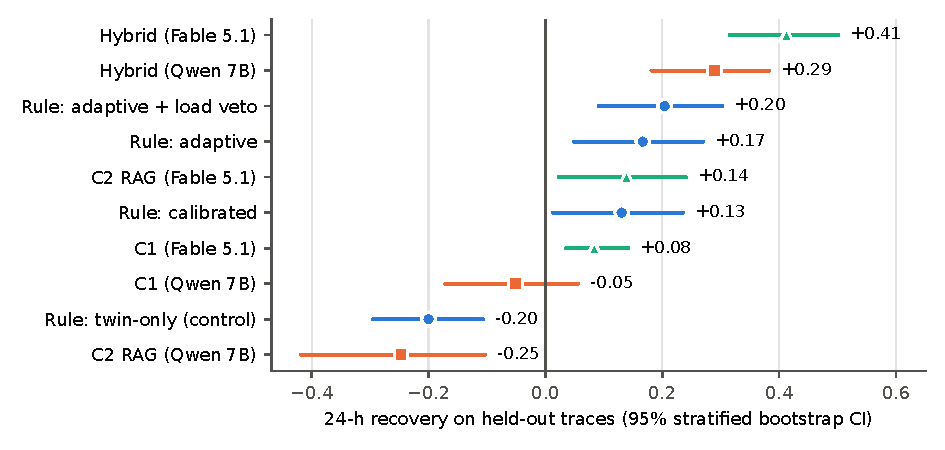
\includegraphics[width=\linewidth]{figures/fig_recovery.pdf}
\caption{Pooled recovery on the held-out traces. Circles: rule-based planners; squares: Qwen2.5 7B; triangles: Claude Fable 5.1.}
\label{fig:recovery}
\end{figure}

With the 7B model, both LLM planners that triage alarms themselves fall far below the rules. C1 behaves like the twin-only heuristic (on the development trace it made the same number of repairs as the twin-only control, with recoveries of $+0.80$ and $+0.78$ on one case and $-0.16$ and $-0.19$ on another), and retrieved knowledge improves it only modestly. Restricting the LLM to vetoing the adaptive rule's candidates (hybrid) reduces the false-alarm cost of the adaptive rule with load veto by about 40\% but acts on the faulty station less often (59 of 72 scenarios against 72).

With the frontier model, the ranking changes. The same C2 design reaches $+0.58$, the highest pooled recovery of all planners, but not by detecting faults more often: it acts on the faulty station in 57 of 72 scenarios, against all 72 for the adaptive rules, with 39 specific hits against 57. Without retrieved knowledge (C1), the frontier model never acts: in all 8\,394 calls it judged every station \emph{insufficient evidence}, reasoning, for example, that \emph{``only the alarm list is available; no transition-time data, trends, or reroutes to distinguish true degradation from known false alarms''}. Its recovery is therefore exactly zero, with no false repairs. Given the same information, the 7B model acts anyway, with 61.6 false repairs per scenario. Figure~\ref{fig:tradeoff} places every planner on the trade-off between recovery under faults and the cost of acting on noise.

\begin{figure}[t]
\centering
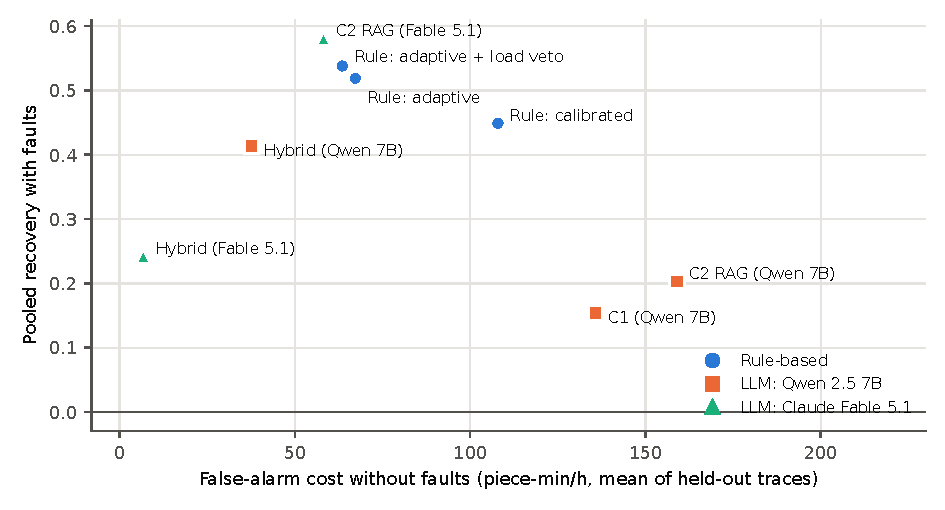
\includegraphics[width=\linewidth]{figures/fig_tradeoff.pdf}
\caption{Recovery with faults against false-alarm cost without faults, held-out traces.}
\label{fig:tradeoff}
\end{figure}

\subsection{Statistical comparison}
Table~\ref{tab:stats} compares C2 on Fable~5.1 with the other planners. Against the best rule, the difference in pooled recovery is $+0.04$, with a 95\% interval from $-0.01$ to $+0.10$; resampling whole traces widens it to $[-0.05, +0.11]$. Per scenario, C2 on Fable~5.1 loses less production time in 50 of 72 scenarios ($p=0.001$, $r=0.43$), but these scenarios are not independent and the gain is uneven across traces: it is ahead on traces 100m--200m ($+0.09$) and 500m--600m ($+0.04$) and behind on 200m--300m ($-0.02$). Against the re-tuned rule, the difference is $+0.04$ $[-0.02, +0.09]$, better in 48 of 72 scenarios. We read the overall result as a match, not a win.

By fault shape (Figure~\ref{fig:shapes}), the two planners are indistinguishable on step and drift faults. On intermittent faults, C2 on Fable~5.1 is better in 21 of 24 scenarios, with $\Delta=+0.21$, but the interval reaches zero ($[0.00, +0.42]$; $[-0.14, +0.47]$ when traces are resampled), 82\% of the piece-minutes it saves on these faults come from trace 100m--200m, and against the re-tuned rule the difference falls to $+0.13$ $[-0.04, +0.30]$. No configuration of the rule grid reaches its $+0.19$ on intermittent faults, so the direction is consistent, but the evidence does not establish an advantage. Nor is it better detection: on intermittent faults the adaptive rules act on the faulty station in all 24 scenarios, C2 on Fable~5.1 in 18.

Timing accounts for most of the pooled difference. The adaptive rules first repair the faulty station a median of 3\,090~min (about two days) after the fault starts; C2 on Fable~5.1, when it acts, after 402~min. In the 57 scenarios where both act, the median paired difference is 0~min ($p=0.17$): most differences are of an hour or two, but in 15 scenarios Fable~5.1 acts more than 1\,000~min earlier, and those 15 account for 96\% of the net piece-minutes it saves. Acting early is not specific to the LLM: the re-tuned adaptive rule without load veto acts after a median of 384~min with the same pooled recovery ($+0.54$). Because recovery is measured over the whole trace (54--168~h), a late first repair of a persistent fault still recovers much of its cost; a plant that needs a response within a shift would weigh the default rule's two-day latency more heavily than this metric does.

\begin{table}[t]
\centering
\caption{C2 (RAG) on Claude Fable 5.1 against other planners, paired over held-out fault scenarios. Wilcoxon $p$-values Holm-adjusted over the rows of each block; $r$: matched-pairs rank-biserial correlation. $\Delta$: difference in pooled recovery (positive favours C2 on Fable 5.1), 95\% bootstrap interval stratified by trace. The breakdown by fault shape is exploratory.}
\label{tab:stats}
\small
\begin{tabular}{lrrrr}
\toprule
Against & Better in & $p$ (Holm) & $r$ & $\Delta$ recovery [95\% CI] \\
\midrule
Adaptive + load veto & 50/72 & 0.001 & 0.43 & $+0.04$ [$-0.01$, $+0.10$] \\
Adaptive rule & 53/72 & $<0.001$ & 0.53 & $+0.06$ [$+0.01$, $+0.13$] \\
Calibrated rule & 63/72 & $<0.001$ & 0.64 & $+0.13$ [$+0.09$, $+0.18$] \\
C2 (RAG), Qwen 7B & 69/72 & $<0.001$ & 0.99 & $+0.38$ [$+0.31$, $+0.47$] \\
C1, Fable 5.1 & 55/72 & $<0.001$ & 0.75 & $+0.58$ [$+0.51$, $+0.64$] \\
\midrule
\multicolumn{5}{l}{\emph{Against rules re-tuned on the development trace}} \\
Adaptive + load veto & 48/72 & 0.022 & 0.31 & $+0.04$ [$-0.02$, $+0.09$] \\
Adaptive rule & 43/72 & 0.016 & 0.36 & $+0.04$ [$-0.01$, $+0.10$] \\
\midrule
\multicolumn{5}{l}{\emph{Against adaptive + load veto, by fault shape}} \\
\quad step & 14/24 & 0.46 & 0.23 & $+0.01$ [$-0.06$, $+0.10$] \\
\quad intermittent & 21/24 & 0.003 & 0.73 & $+0.21$ [$\phantom{+}0.00$, $+0.42$] \\
\quad drift & 15/24 & 0.46 & 0.29 & $+0.02$ [$-0.06$, $+0.10$] \\
\bottomrule
\end{tabular}
\end{table}

\begin{figure}[t]
\centering
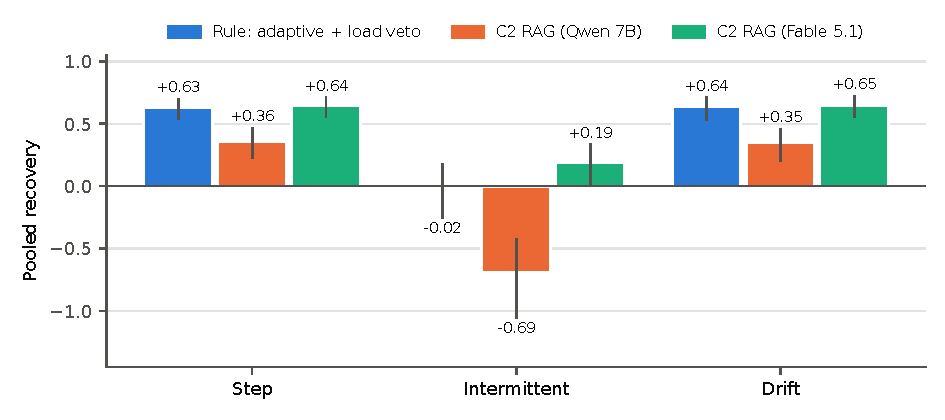
\includegraphics[width=\linewidth]{figures/fig_shapes.pdf}
\caption{Pooled recovery by fault shape on the held-out traces (24 scenarios per shape). Whiskers: 95\% bootstrap interval stratified by trace.}
\label{fig:shapes}
\end{figure}

\subsection{The hybrid and the batched-alarm artefact}
The hybrid behaves in the opposite way with the frontier model: it becomes extremely conservative (5.1 false repairs per scenario, false-alarm cost 7 piece-min/h) and acts on the faulty station in only 34 of 72 scenarios. Fable~5.1 vetoed at least one station in 1\,256 of its 1\,437 calls. Coded with an explicit keyword rule (\emph{burst}, \emph{line-wide}, \emph{common cause}, \emph{systemic}; rule and counts in the repository), 98\% of those vetoes, and all 167 vetoes of a station that was actually faulty, argue that the alarms come in bursts shared by many stations and therefore point to a common, line-wide cause. For example, with L0\_S4 faulty: \emph{``Every alarm is a line-wide burst (all L0 stations plus L3) with twins alarming together; points to a common upstream cause, not individual faults. Hold off.''} The premise is an artefact of the detector: it raises an alarm \emph{only} when more than 10\% of the stations are flagged in the same batch, so every alarm it produces is, by construction, a shared burst. The hybrid's prompt, however, names such bursts among the contexts that may justify doubting the test, and the system prompt describes the batch rule. With the same prompt, the 7B model uses this argument in 1\% of its vetoes (33\% mention shared alarms at all, often while still concluding that the station is degraded). The stated reasons are therefore consistent with a capable model applying a cue we provided to evidence whose structure the detector imposes. They do not show that the model discovered the artefact, nor do they separate reasoning from closer instruction following; a run without that cue would be needed to identify the mechanism.

% =====================================================================
\section{Discussion}
\label{sec:discussion}

\paragraph{The bottleneck is triage, not planning}
Once a station is correctly judged faulty, a simple rule (reroute to a free twin, repair) is enough in our action space. The differences we measured between planners come from deciding which alarms deserve action, and when. Closing the loop on the 2020 system without triage would have repaired dozens of healthy stations per fault for no net gain.

\paragraph{A frontier model matches a good statistical test; a 7B model does not}
The same retrieval-augmented design goes from $+0.20$ to $+0.58$ when the 7B model is replaced by the frontier model. This is a contrast between two systems, which differ in size, quantisation, provider and inference settings, not a measured capability curve. The two models also use retrieval differently. Without it, the 7B model acts on alarms it cannot assess, and retrieval improves it only from $+0.15$ to $+0.20$; the frontier model declines to act, and retrieval is what turns that abstention into $+0.58$. For a capable model, the Knowledge component is not an optional refinement but the condition for acting. At its best, the LLM planner matches a well-tuned change test, which is cheaper, faster to evaluate and fully reproducible. On intermittent faults, whose on--off pattern dilutes alarm rates, it is ahead of every rule configuration we tried; this direction deserves testing on more traces, not a claim of superiority.

\paragraph{The Analyze--Knowledge interface shapes the planner}
As a veto over the legacy detector, the frontier model was less useful than the 7B model, and its reasons rest on the batched structure of the alarms. Whatever the exact mechanism, in MAPE-K terms the information passed from Analyze to Plan (batched alarms) does not carry the per-station evidence a planner needs to tell a degraded station from a line-wide disturbance. The implication for the architecture is to pass per-station evidence rather than batched alarms, and to test that change before investing in more capable planners.

\paragraph{Implications for practice}
Within the limits of a study with synthetic faults, three points transfer to automation architects and maintenance engineers. First, connecting threshold alarms directly to maintenance orders is at best useless and at worst harmful, because false repairs accumulate; alarms must be rationalised before they drive actions, as alarm-management practice already requires for operators~\cite{isa182}. Second, a rate-change test over each station's own recent history is a cheap and transparent triage layer, and the reference that any learned or LLM-based controller should be compared with. Third, its window is a design parameter: a short window responds within a shift at the same recovery. An LLM planner can perform at the same level, but its non-determinism and its sensitivity to how alarms are presented argue for keeping it advisory, with every action passing a symbolic validator, as here, and, in a plant, human approval.

\paragraph{Development sets mislead}
On the development trace, three conclusions were wrong: the 7B retrieval-augmented planner appeared to beat the calibrated rule, the hybrid appeared to match its control at a lower false-alarm cost, and the frontier model appeared equivalent to the 7B model. Only the held-out traces reversed them. The development cases contained no intermittent fault, the shape on which the held-out results differ most. A single trace with four cases is too small to select designs on, and LLM-based controllers should be evaluated on data not used to write their prompts.

\paragraph{Threats to validity}
\emph{Construct}: faults are synthetic, and the effect model is additive and trace-driven, without queueing, so every recovery is a property of the model, not a measured property of the Bosch line. Its unverifiable parameters were swept one at a time, for rules on step faults only: the congestion parameter does not change any conclusion, but mild faults, long repairs and stop-mode maintenance reduce or reverse the benefit of triage, and no sensitivity analysis was run for the LLM planners. Recovery is measured in production time over the whole trace, without economic weights, and therefore values a late repair of a persistent fault. \emph{Internal}: the specific-hit metric depends on a $\pm$120~min window (with $\pm$60 and $\pm$240~min, C2 on Fable~5.1 scores 44 and 37 of 72, the adaptive rules 57 and 57); each frontier-model decision is a single stored sample at low effort, and 78\% of its calls reuse a stored response; the prompts are part of the treatment, and the hybrid's prompt contains the cue its vetoes cite; the 7B model is 4-bit quantised. The frontier model may have seen our 2020 papers, which name the Bosch line, but the faults are synthetic and not described anywhere it could have seen. \emph{External}: one production line, one dataset and one legacy detector; two language models, with no intermediate sizes. \emph{Statistical}: scenarios on the same trace are not independent; three held-out traces are few clusters, and the trace-level bootstrap gives wider intervals than the stratified one.

% =====================================================================
\section{Conclusion}
\label{sec:conclusion}

We closed the autonomic loop of a self-coordinated manufacturing architecture that, as published, only detected. Doing so naively brings no benefit, because the decisive problem is alarm triage. A classical adaptive change test is a strong baseline, and re-tuning it does not change that. A frontier LLM with retrieved operational knowledge matches it, while the same design on a 7B model does not; on intermittent faults it is ahead of every rule we tried, an exploratory result that needs more traces. Used as a veto over batched alarms, the frontier model becomes overly conservative, citing the line-wide structure that the detector imposes on every alarm. Future work will redesign the Analyze--Knowledge interface to pass per-station evidence, run the hybrid without the burst cue, add intermediate model sizes and repeated samples, and validate the effect model against plant data with real capacities and repair times.

% =====================================================================
\section*{Data and code availability}
\label{sec:availability}
The headless simulator, planners, prompts, development log, every model decision with its stated reason, the results and the scripts that produce every table and figure are available at \url{https://github.com/mbsanchez/ssacsimulator}. The simulator uses the Python standard library only; the statistics and figures additionally use SciPy and matplotlib. The Bosch dataset is publicly available~\cite{bosch2016kaggle}; the files derived from it (process model and event traces) are not redistributed, and the repository gives the scripts that produce them and their checksums.

\section*{CRediT authorship contribution statement}
\textbf{Manuel S\'anchez:} Conceptualization, Methodology, Investigation, Visualization, Writing -- original draft. \textbf{Ernesto Exposito:} Supervision, Writing -- review \& editing.

\section*{Declaration of competing interest}
The authors declare that they have no known competing financial interests or personal relationships that could have appeared to influence the work reported in this paper.

\section*{Declaration of generative AI and AI-assisted technologies in the manuscript preparation process}
During the preparation of this work the authors used Claude (Anthropic) to assist in developing the simulation and analysis software, to draft and revise the text of the manuscript, and as an adversarial agent acting as a peer reviewer to identify weaknesses and suggest improvements. The software was reviewed by the first author. After using this tool, the authors reviewed and edited the content as needed and take full responsibility for the content of the published article. The use of Qwen2.5 and Claude Fable~5.1 as planners is part of the method studied in this paper (Section~\ref{sec:planners}) and is unrelated to the preparation of the manuscript.

\bibliographystyle{elsarticle-num}
\bibliography{refs}

\end{document}
